\documentclass[12pt, a4paper]{article}

% ── Packages ──────────────────────────────────────────────────────────────────
\usepackage{amsmath, amssymb, amsthm}
\usepackage{geometry}
\usepackage{booktabs}
\usepackage{array}
\usepackage{hyperref}
\usepackage{xcolor}
\usepackage{tcolorbox}
\usepackage{enumitem}
\usepackage{parskip}
\usepackage{tikz}
\usetikzlibrary{arrows.meta, positioning, calc}

\geometry{margin=2.5cm}

% ══════════════════════════════════════════════════════════════════════════════
% ── Student-mode switch ───────────────────────────────────────────────────────
%
%   \studentmodetrue  → student version: blanks replace selected equations
%   \studentmodefalse → instructor version: all equations shown in full
%
\newif\ifstudentmode
\studentmodefalse       % default: instructor mode

\ifx\studentflag\undefined
  % no flag passed — keep studentmodefalse
\else
  \studentmodetrue
\fi
% ══════════════════════════════════════════════════════════════════════════════

% ── Student-mode macros ───────────────────────────────────────────────────────
\newcommand{\sol}[2][6cm]{%
  \ifstudentmode
    \underline{\hspace{#1}}%
  \else
    {#2}%
  \fi
}

\newcommand{\soleq}[2][3cm]{%
  \ifstudentmode
    \par\vspace{4pt}%
    \noindent\rule{\linewidth}{0.5pt}\\[#1]%
    \noindent\rule{\linewidth}{0.5pt}%
    \par\vspace{4pt}%
  \else
    \[#2\]%
  \fi
}
% ──────────────────────────────────────────────────────────────────────────────

% ── Colors & boxes ────────────────────────────────────────────────────────────
\definecolor{mainblue}{RGB}{30, 100, 180}
\definecolor{boxbg}{RGB}{235, 243, 255}
\definecolor{notebg}{RGB}{255, 248, 230}
\definecolor{warnbg}{RGB}{255, 235, 235}

\tcbuselibrary{skins, breakable}

\newtcolorbox{resultbox}{
  colback=boxbg, colframe=mainblue,
  boxrule=1.2pt, arc=4pt,
  title={Result},
  fonttitle=\bfseries\color{white},
  coltitle=white, attach boxed title to top left={yshift=-2mm, xshift=4mm},
  boxed title style={colback=mainblue, arc=3pt}
}

\newtcolorbox{notebox}{
  colback=notebg, colframe=orange!70!black,
  boxrule=1pt, arc=4pt,
  left=4pt, right=4pt
}

\newtcolorbox{warnbox}{
  colback=warnbg, colframe=red!60!black,
  boxrule=1pt, arc=4pt,
  left=4pt, right=4pt
}
% ──────────────────────────────────────────────────────────────────────────────

% ── Theorem environments ───────────────────────────────────────────────────────
\theoremstyle{definition}
\newtheorem{example}{Example}[section]

% ── Math macros ───────────────────────────────────────────────────────────────
\newcommand{\yhat}{\hat{y}}
\newcommand{\pd}[2]{\dfrac{\partial #1}{\partial #2}}

% ── Document ──────────────────────────────────────────────────────────────────
\begin{document}

\begin{center}
  {\LARGE \textbf{Section 3.2: Gradient Descent}} \\[0.3em]
  {\large\itshape How Machines Learn by Walking Downhill} \\[0.5em]
  {\large AI Class --- Lecture Notes}%
  \ifstudentmode
    \quad {\normalsize\color{gray}[Student Copy]}%
  \fi
\end{center}

\vspace{1em}
\hrule
\vspace{1.5em}

% ══════════════════════════════════════════════════════════════════════════════
\section{Why We Need a New Strategy}

In Section 1.1 (linear regression) we minimised the MSE loss by setting
$\partial J/\partial w = 0$ and solving analytically.  This gave a clean,
exact answer in one step --- the \emph{normal equations}.

But that only works because the loss was a simple convex quadratic in $w$.
For a neural network the loss depends on weights through several layers of
non-linear activation functions.  Setting all partial derivatives to zero
produces a system of equations with \textbf{no closed-form solution}.

We therefore need an \textbf{iterative} approach:
\begin{enumerate}[nosep]
  \item Start with some initial guess for the weights.
  \item Compute how the loss changes with each weight (the gradient).
  \item Nudge every weight in the direction that reduces the loss.
  \item Repeat until the loss stops improving.
\end{enumerate}

This procedure is called \textbf{gradient descent}, and it is the foundation
of virtually all modern machine-learning optimisers.

% ══════════════════════════════════════════════════════════════════════════════
\section{The Gradient as a Compass}

Recall that for a function $J(w)$, the derivative $dJ/dw$ measures the
\emph{slope} of $J$ at the current value of $w$:

\begin{center}
\renewcommand{\arraystretch}{1.3}
\begin{tabular}{cl}
\toprule
Sign of $dJ/dw$ & Meaning \\
\midrule
$> 0$ & $J$ rises as $w$ increases $\;\Rightarrow\;$ \textbf{decrease} $w$ \\
$< 0$ & $J$ falls as $w$ increases $\;\Rightarrow\;$ \textbf{increase} $w$ \\
$= 0$ & $J$ is flat here $\;\Rightarrow\;$ we are at a (local) minimum \\
\bottomrule
\end{tabular}
\end{center}

Both non-zero cases are captured by a single rule: subtract a small multiple
of the gradient from the current weight.

\begin{resultbox}
\textbf{Gradient Descent Update Rule}
\[
  w \;\longleftarrow\; w \;-\; \eta\,\frac{dJ}{dw}
\]
where $\eta > 0$ (pronounced ``eta'') is the \textbf{learning rate}: a small
positive constant controlling the step size.
\end{resultbox}

Applying this update repeatedly is called \textbf{gradient descent} because
we are literally descending the loss surface step by step.

% ══════════════════════════════════════════════════════════════════════════════
\section{A Hand-Calculated Example}

\begin{example}
\textbf{Setup.}
One training point: $x = 2$, $y = 4$.
Model (no bias): $\yhat = wx$.
Loss:
\[
  J(w) = (y - wx)^2 = (4 - 2w)^2.
\]
The true weight is clearly $w^{*} = 2$, since $\yhat = 2 \times 2 = 4 = y$.
We start at $w_0 = 0$ and run gradient descent with learning rate
$\eta = 0.1$.
\end{example}

% ──────────────────────────────────────────────────────────────────────────────
\subsection{Deriving the Gradient}

Differentiate $J(w) = (4 - 2w)^{2}$ with respect to $w$ using the chain rule:

\[
  \frac{dJ}{dw}
  = 2\,(4 - 2w)\cdot(-2)
  = \sol[5cm]{-4\,(4 - 2w)}
\]

At $w = 0$:
\[
  \left.\frac{dJ}{dw}\right|_{w=0}
  = -4\,(4 - 0)
  = \sol[3cm]{-16}
\]

The gradient is \emph{negative}, telling us that $J$ decreases as $w$
increases --- so the update will increase $w$.  That makes sense: we need to
move from $w=0$ towards $w^{*}=2$.

% ──────────────────────────────────────────────────────────────────────────────
\subsection{Four Update Steps}

Apply $w \leftarrow w - 0.1\,\dfrac{dJ}{dw}$ repeatedly, using
$\dfrac{dJ}{dw} = -4(4-2w)$ each time:

\vspace{0.5em}
\begin{center}
\renewcommand{\arraystretch}{2.0}
\begin{tabular}{c >{\centering}p{1.4cm} >{\centering}p{2.2cm}
                  >{\centering}p{4.0cm} p{4.0cm}}
\toprule
Step $t$ & $w_t$ & $J(w_t)$ & $dJ/dw$ at $w_t$
         & $w_{t+1} = w_t - 0.1\,\cdot\,dJ/dw$ \\
\midrule
0 & $0$     & \sol[1.6cm]{$16$}    & \sol[3.0cm]{$-4(4-0)=-16$}      & \sol[3.5cm]{$0-0.1(-16)=1.6$} \\
1 & $1.6$   & \sol[1.6cm]{$0.64$}  & \sol[3.0cm]{$-4(0.8)=-3.2$}     & \sol[3.5cm]{$1.6-0.1(-3.2)=1.92$} \\
2 & $1.92$  & \sol[1.6cm]{$0.026$} & \sol[3.0cm]{$-4(0.16)=-0.64$}   & \sol[3.5cm]{$1.92-0.1(-0.64)=1.984$} \\
3 & $1.984$ & \sol[1.6cm]{$0.001$} & \sol[3.0cm]{$-4(0.032)=-0.128$} & \sol[3.5cm]{$1.984-0.1(-0.128)\approx 1.997$} \\
\bottomrule
\end{tabular}
\end{center}
\vspace{0.5em}

After only four steps from $w_0 = 0$, the weight has reached $1.997$ ---
within $0.15\%$ of the true value $w^{*} = 2$.
Note that the gradient shrinks at each step, so the updates automatically
become smaller as we approach the minimum.

% ──────────────────────────────────────────────────────────────────────────────
\subsection{Visualising the Descent}

\begin{center}
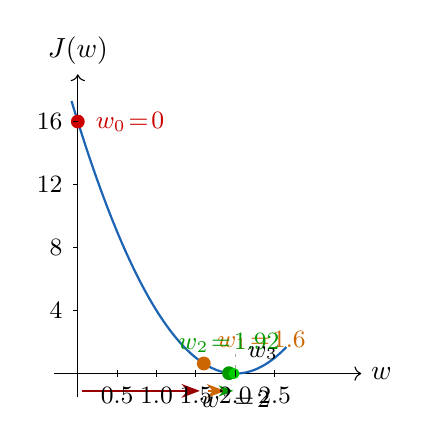
\begin{tikzpicture}[scale=1.0]
  % ── Axes ──────────────────────────────────────────────────────────────────
  \draw[->] (-0.3, 0) -- (3.6, 0) node[right] {$w$};
  \draw[->] (0, -0.3) -- (0, 3.8) node[above] {$J(w)$};

  % ── Parabola: J(w)=(4-2w)^2, plotted as y=(4-2x)^2/5 for x in [-0.1,2.7] ─
  \draw[thick, mainblue, domain=-0.08:2.65, samples=120]
    plot (\x, {(4 - 2*\x)^2 / 5});

  % ── Minimum marker ────────────────────────────────────────────────────────
  \draw[dashed, gray!70] (2, 0) -- (2, 0.25);
  \node[below] at (2, -0.08) {\small $w^*\!=\!2$};

  % ── Step points (x = w, y = J/5) ─────────────────────────────────────────
  % w0=0:    J=16,     y=3.20
  % w1=1.6:  J=0.64,   y=0.128
  % w2=1.92: J=0.026,  y≈0.005
  % w3=1.984:J=0.001,  y≈0.0002
  \fill[red!80!black]      (0,   3.20)  circle (2.5pt);
  \fill[orange!80!black]   (1.6, 0.128) circle (2.5pt);
  \fill[green!60!black]    (1.92,0.005) circle (2.5pt);
  \fill[green!80!black]    (1.984,0.0002) circle (2pt);

  % ── Labels ────────────────────────────────────────────────────────────────
  \node[right=3pt, red!80!black]    at (0,   3.20)  {\small $w_0\!=\!0$};
  \node[above right=2pt, orange!80!black] at (1.6, 0.128) {\small $w_1\!=\!1.6$};
  \node[above=4pt, green!60!black]  at (1.92,0.005) {\small $w_2\!=\!1.92$};
  \node[above right=2pt]            at (1.984,0.0002){\small $w_3$};

  % ── Progress arrows along x-axis ─────────────────────────────────────────
  \draw[-{Stealth[scale=1.0]}, thick, red!60!black]
    (0.05, -0.22) -- (1.55, -0.22);
  \draw[-{Stealth[scale=1.0]}, thick, orange!80!black]
    (1.65, -0.22) -- (1.87, -0.22);
  \draw[-{Stealth[scale=0.8]}, thick, green!60!black]
    (1.925,-0.22) -- (1.975,-0.22);

  % ── Y-axis ticks ─────────────────────────────────────────────────────────
  \foreach \jval/\ypos in {4/0.8, 8/1.6, 12/2.4, 16/3.2} {
    \draw (-0.06, \ypos) -- (0, \ypos)
      node[left=2pt] {\small \jval};
  }

  % ── X-axis ticks ─────────────────────────────────────────────────────────
  \foreach \xval in {0.5, 1.0, 1.5, 2.0, 2.5} {
    \draw (\xval, 0.05) -- (\xval, -0.05)
      node[below] {\small \xval};
  }
\end{tikzpicture}
\end{center}

The dots show the position of $w_t$ on the loss curve at each step.
Each step is smaller than the last because the gradient --- and hence the
slope of the curve --- becomes flatter as we near the bottom.

% ══════════════════════════════════════════════════════════════════════════════
\section{The Learning Rate $\eta$}

The learning rate $\eta$ controls how large each step is.
Choosing it well is important: too small and training is painfully slow;
too large and the updates overshoot the minimum.

% ──────────────────────────────────────────────────────────────────────────────
\subsection*{Too Small: $\eta = 0.01$}

Using the same example, first update:
\[
  w_1 = 0 - 0.01 \times (-16) = \sol[2cm]{0.16}
\]
The algorithm will still converge to $w^* = 2$, but it now needs roughly
ten times as many steps.

% ──────────────────────────────────────────────────────────────────────────────
\subsection*{Too Large: $\eta = 0.5$}

First update:
\[
  w_1 = 0 - 0.5 \times (-16) = \sol[2cm]{8.0}
\]

The weight \emph{overshoots} past $w^* = 2$ all the way to $8$.
Check what happens next:

\[
  \left.\frac{dJ}{dw}\right|_{w=8}
  = -4(4 - 16) = \sol[2.5cm]{48}
  \qquad\Rightarrow\qquad
  w_2 = 8 - 0.5 \times 48 = \sol[2cm]{-16}
\]

The loss is now \emph{larger} than it was at $w_0 = 0$, and the updates
will keep growing.  The algorithm \textbf{diverges}.

\begin{warnbox}
\textbf{Symptom of a bad learning rate:} if $J$ increases during training,
$\eta$ is almost certainly too large.  A safe starting point for most
problems is $\eta = 0.01$.
\end{warnbox}

% ══════════════════════════════════════════════════════════════════════════════
\section{From One Weight to a Neural Network}

Everything above applies to a network with many weights.
Suppose the network has weight matrices $\mathbf{W}^{(1)}, \mathbf{W}^{(2)}$
and biases $\mathbf{b}^{(1)}, \mathbf{b}^{(2)}$.
After every forward pass we apply:

\[
  W_{ij}^{(\ell)} \;\longleftarrow\;
  W_{ij}^{(\ell)} - \eta\,\frac{\partial J}{\partial W_{ij}^{(\ell)}}
  \qquad \text{for every layer } \ell \text{ and every entry } (i,j).
\]

The structure is identical to the 1-weight example --- only the number of
updates differs.

The sole new challenge is \emph{computing}
$\partial J / \partial W_{ij}^{(\ell)}$ for each weight.
Because the loss depends on a weight only indirectly --- through several
layers of non-linear activation functions --- these gradients are not
obvious to write down.

\begin{notebox}
\textbf{Coming next.}
In Section 3.3 we build a concrete two-layer network and trace a prediction
step by step (the \emph{forward pass}).  In Section 3.4 we derive the
gradients by working backwards through the same network
(the \emph{backward pass}, or \textbf{backpropagation}).
Only then will we have everything needed to run gradient descent on a
neural network.
\end{notebox}

\end{document}
